\documentclass[paper=a4, fontsize=11pt]{scrartcl}
\usepackage[T1]{fontenc}
\usepackage{fourier}

\usepackage[english]{babel}                             % English language/hyphenation
\usepackage[protrusion=true,expansion=true]{microtype}
\usepackage{amsmath,amsfonts,amsthm} % Math packages
\usepackage[pdftex]{graphicx}
\usepackage{url}
\usepackage{gensymb}
\graphicspath{{/home/chris/machine_learning_final_project/keras/}}
%%% Begin document

\begin{document}
\section*{Methodology and Results}
\subsection*{Ensemble Methods}
\subsubsection*{Boosting}

In order to choose the hyperparameters, grid search cross-validation is implemented on training data.
For the grid search cross-validation, we consider the number of trees, the max-depth of each tree and also the sample size of feasures for building each individual tree.
The grid is:

\begin{table}[ht]
\centering
\caption{Grid Search CV for Boosting}
\label{my-label}
\begin{tabular}{llll}
\hline
\textit{number of rounds:} & 100 & 500 & 1000 \\
\textit{feature proportion:}     & 0.3 & 0.8 & 1   \\
\textit{maximum depth:}    & 6   & 9   & 12  \\ \hline
\end{tabular}
\end{table}

Actually, there are several different combination that give us almost the same prediction accuracy. Hence, we choose the simplest one among them, where number of rounds is 100, feature proportion $100\%$, and maximum depth is 6.

More, we use three measures to evalutate the model, which is f1-score, precision and recall.
The three measures are defined as follow:
\[precison = \frac{{tp}}{{tp + fp}}\]
\[recall = \frac{{tp}}{{tp + fn}}\]
\[F = 2\frac{{precison \times recall}}{{precison + recall}}\]

where \textit{tp} is true positive, \textit{fp} is false postive,and \textit{fn} is false negative. For multiclass classification problem, we take class C as example. True positive is the diagnoal position in confusion matrix cm(C, C). False positive is sum of column C(without main diagonal). False negative is sum of row C (without main diagonal)

\begin{table}[ht]
\centering
\caption{Summary for Boosting}
\begin{tabular}{lllll}
\hline
            & precision & recall & f1-score & support \\ \hline
0           & 0.83      & 0.86   & 0.84     & 177     \\
1           & 0.78      & 0.87   & 0.82     & 139     \\
2           & 0.95      & 0.92   & 0.93     & 163     \\
3           & 0.77      & 0.73   & 0.75     & 136     \\
4           & 0.85      & 0.82   & 0.83     & 179     \\
5           & 0.75      & 0.71   & 0.73     & 141     \\
6           & 0.96      & 0.96   & 0.96     & 395     \\
7           & 0.66      & 0.68   & 0.67     & 135     \\ \hline
avg / total & 0.85      & 0.85   & 0.85     & 1465    \\ \hline
\end{tabular}
\end{table}
\newpage
And the total prediction accuracy for the model 0.8464. From the three measures, the prediction performance for different classes are not balanced.


\subsubsection*{Random Forest}

\begin{table}[ht]
\centering
\caption{Grid Search CV for Random Forest}
\begin{tabular}{llll}
\hline
\textit{number of trees:} & 100 & 500 & 1000 \\
\textit{maximum feature:}     &200  & 500 & 1000   \\
\textit{maximum depth:}    & 6   & 9   & 12  \\ \hline
\end{tabular}
\end{table}
We evaluate the model by their prediction accuracy, and the best model is: number of trees is 500; maximum features is 200; maximum depth for base classifier is 9.

We also use the three measures to evaluate our model in details.

\begin{table}[ht]
\centering
\caption{Summary for Random Forest}
\begin{tabular}{lllll}
\hline
            & precision & recall & f1-score & support \\ \hline
0           & 0.72      & 0.90   & 0.80     & 177     \\
1           & 0.88      & 0.81   & 0.85     & 139     \\
2           & 0.97      & 0.94   & 0.95     & 163     \\
3           & 0.83      & 0.74   & 0.78     & 136     \\
4           & 0.81      & 0.80   & 0.81     & 179     \\
5           & 0.78      & 0.74   & 0.76     & 141     \\
6           & 0.98      & 0.96   & 0.97     & 395     \\
7           & 0.71      & 0.72   & 0.72     & 135     \\ \hline
avg / total & 0.86      & 0.85   & 0.86     & 1465    \\ \hline
\end{tabular}
\end{table}

And the total prediction accuracy for the model 0.8546. From the three measures, the prediction performance for different classes are not balanced. Moreover, for ensemble methods, Random Forest are somehow better than Boosting in terms of prediction performance in average.

\subsubsection*{Ensemble Methods with Pretraining}
For this part, two models for pretraining are considered: Restricted Bolzmann Machine(RBM) and Deep Belief Network(DBN). We firstly scale the data to 0-1 in order to learned the distribution for data based on Bernoulli distribution. Secondly, we implement the two models in order to learn the new feature representations. Thirdly the Ensemble Methods are trained by these reconstructed training data. For prediction, we also transform the original data and then do prediction. However, the results are not satisfactory. The reason may be that the distribution for our data are not easily learned by Bernoulli RBM or DBN.

\subsubsection*{Conclusion for Ensemble Methods}
The performance for different Ensemble Methods are almost the same. The prediction accuracies for the two models are both around 85\%. However, further improvement cannot be achieved even more base classifers are incorporated. From this point of view, we think that we've already reached the limitation of ensemble methods for this particular problem.

\subsection*{Convolutional Neural Networks}
\subsubsection*{Data Augmentation}
For this part, the \textit{Real-Time Data Augmentation} is applied. Specifically, for each mini-batch, we modify the inputs following some specified methods, the degrees of modification are decided randomly. In other words, we always keep original images. Through the optimization process, we always use their modified version which is randomly decided by the algorithm. The advantages of \textit{Real-Time Data Augmentation} are as follows: firstly, it greatly saves the space for data storage, because we only keep the original images and modified versions are threw away once we finish one minibatch; secondly, the data augmentation is accomplished through the optimization, so for each epoch we always use different data(randomly modified version of original data), which means the degree of data augmentation is simply decided by how many epoches we run.

\textbf{Affine Transformations}:

\textbf{rotation:} randomly rotate images in the range($0^\circ$, 180\degree) uniformly with step length 20\degree

\textbf{width shift:} randomly shift images horizontally following Bernoulli distribution p = 0.5 by 20\% of total width

\textbf{height shift:} randomly shift images vertically following Bernoulli distribution p = 0.5 by 20\% of total height

\textbf{horizontal flip} randomly flip image horizontally following Bernoulli distribution p = 0.5

\subsubsection*{Layer Building}
The size of our minibatch is $32$, and for each image, it's actually an 3D array (1,32,32). \textit{1} stands for only one channel, and $32 \times 32$ stands for the dimension of the image's pixels.  The kernels for the Convolutional Neural Network are all with the dimension $3 \times 3$. For Layer activation, we take Rectified Linear Units(ReLU) as our activation function, which is always implemented after each convolution layer. \textit{Dropout} technique is also adopted for the sake of optimization efficiency and robustness after each max-pooling layer. The activation function for our fully connected is also ReLU. The loss function for the Convolutional Neural Networks is \textit{Softmax} function, which is the common choice for multiclass classification problem.

The structure of the Convolutional Neural Network is as follows:
\begin{table}[ht]
\centering
\caption{Structure For Convolutional Neural Network}
\begin{tabular}{lll}
\hline
\textit{\textbf{Layer}}  & \textit{\textbf{Size}}                                                     & \textit{\textbf{Output shape}} \\ \hline
\textit{input}           &                                                                                    & (32, 1, 32, 32)                \\
\textit{convolution}     & 32 3x3 filters                                                                     & (32, 32, 32, 32)               \\
\textit{convolution}     & 32 3x3 filters                                                                     & (32, 32, 32, 32)               \\
\textit{max-pooling}     & \begin{tabular}[c]{@{}l@{}}2x2, stride 2\\ followed by 0.25 dropout\end{tabular}   & (32, 32, 16, 16)               \\
\textit{convolution}     & 64 3x3 filters                                                                     & (32, 64, 16, 16                \\
\textit{convolution}     & 64 3x3 filters                                                                     & (32, 64, 16, 16)               \\
\textit{max-pooling}     & \begin{tabular}[c]{@{}l@{}}2x2, stride 2\\ followed by 0.25 dropout\end{tabular}   & (32, 64, 8, 8)                 \\
\textit{fully connected} & \begin{tabular}[c]{@{}l@{}}512 hidden units\\ followed by 0.5 dropout\end{tabular} & (32,512)                       \\
\textit{fully connected} & 8 way soft-max                                                                     & (32,8)                         \\ \hline
\end{tabular}
\end{table}

\newpage
\subsubsection*{Prediction Performance}
Firstly, we display the curve of prediction accuracy for test set w.r.t epoch, \textit{1000} epoches are run for optimization.
\begin{figure}[ht]
\centering
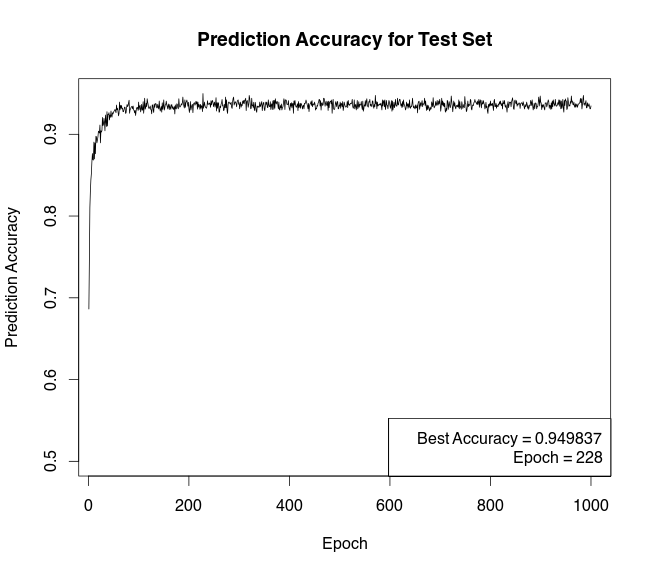
\includegraphics[width=6cm,height=6cm,angle=0]{Rplot.png}
\end{figure}
From the plot, we see that the prediction performance of Convolutional Neural Network wiggle around an certain level after almost 20 epoches. The best prediction accuracy is achieved at \textit{Epoch 228} with accuracy 0.949837, and it maintains above 0.9 after {Epoch 20}. The algorithm almost converges after 50 epoches. Here we only display the summary for the classifier after 1000 epoches.

The prediction performance for each class:
\begin{table}[ht]
\centering
\caption{Summary for Convolutional Neural Network}
\begin{tabular}{lllll}
\hline
            & precision & recall & f1-score & support \\ \hline
0           & 0.99      & 0.97   & 0.98     & 177     \\
1           & 0.97      & 0.97   & 0.97     & 139     \\
2           & 0.95      & 0.99   & 0.97     & 163     \\
3           & 0.96      & 0.93   & 0.94     & 136     \\
4           & 0.96      & 0.96   & 0.96     & 179     \\
5           & 0.78      & 0.82   & 0.80     & 141     \\
6           & 0.96      & 0.97   & 0.97     & 395     \\
7           & 0.85      & 0.79   & 0.82     & 135     \\ \hline
avg / total & 0.94      & 0.94   & 0.94     & 1465    \\ \hline
\end{tabular}
\end{table}

The total prediction accuracy after 1000 epoches is 0.9365, The prediction accuracy for each class is much more balanced than previous methods. We can see that the Convolutional Neural Network can handle different classes well.

\section*{Conclusion}
The prediction preformance of Convolutional Neural Network(accuracy = 95\%) is much better than Ensemble Method (accuracy = 85\%) for this image recognition problem, which justifies the advantage of CNN in this specific field. The good performance of Convolutional Neural Network is firstly decided by its model complexity, which is quite approriate for image recognition problem. In other words, large data set and huge feature dimension are kinds of prerequisite for the usage of Convolutional Neural Network. Moreover, the success of Convolutional Neural Network is also decided by that it captures the local structures for images, which is one of the most significant characteristics of image data. This advantage is based on the fact that convolution layer enable the local data to share the weights, which is quite different from other methods. In conclusion, Convolutional Neural Network has great advantages in image recognition problem.


\section*{Appendix}
For Ensemble Methods, we firstly vectorzie the image and save it as .npy file. For the Convolutional Neural Network, we store the file as 4D array (d1, d2, d3, d4), where d1 stands for the number of observations, d2 stands for the number of channels, $d1 \times d2$ stands for the dimension for pixels.
We use several python modules for this project, including sklearn, Theano, xgboost and keras. The sklearn module is used for Random Forest and Restricted Bolzmann Machine pretraining. Theano is implemented for training the Deep Network Network. The xgboost module is taken to realize the boosting algorithm. Finally, we use keras to solve the Convolution Neural Network problem with real-time data augmentation.

\end{document}


